\section{Satellite Galaxies Around a Massive Central}

\lstinputlisting[caption={Code for all the algorithms used in this exercise}, linerange={10, 245}]{ancillary.py}
\lstinputlisting[caption={Code for the random number generator}, firstline={3}]{rng.py}

All dynamically written results from the code corresponding to this section can be found in \texttt{results/satellite\_galaxies\_results.txt}.

In this section we will investigate the spherical distribution of satellite galaxies around a massive central galaxies. Their density distribution $n$ can be described

\begin{equation}
    n(x) = A\left<N_{sat}\right>\left(\frac{x}{b}\right)^{a-3}\exp{\left[-\left(\frac{x}{b}\right)^{c}\right]}\label{eq:nx}
\end{equation}

Where we take $a = 2.4$, $b = 0.25$, $c = 1.6$ and $\left<N_{sat}\right> = 100$. $x$ is the radius relative to the virial radius, i.e. $x \equiv r/r_{vir}$. $A$ is a normalization constant that we do not a priori know, but is set such that the three dimensional spherical from $x = 0$ to $x_{max} = 5$ is equal to the average number of satellites, $\left<N_{sat}\right>$:

\begin{equation}
    \int\int\int_V n(x)dV = \left<N_{sat}\right>.\label{eq:vol_int}
\end{equation}

\lstinputlisting[caption={Setup code for the first assignment}, linerange={8 -11, 18-34}]{satellite_galaxies.py}

\subsection{Normalization Constant}

Looking at equation \ref{eq:nx} we can see that it is independent of angle, and only depends on the radial distance. This allows us to transform the integral in equation \ref{eq:vol_int} to a spherical integral over $\theta, \phi, x$ as

\begin{align*}
    \int\int\int_V n(x)dV &= \int_0^{x_{max}} \int_0^{\pi} \int_0^{2\pi} n(x)x^2\sin(\theta) d\phi d\theta dx \\
& = 4\pi~\int_0^{x_{max}} n(x)x^2 dx \\
&= 4\pi~\int_0^{x_{max}} x^2 A\left<N_{sat}\right>\left(\frac{x}{b}\right)^{a-3}\exp{\left[-\left(\frac{x}{b}\right)^{c}\right]} dx
\end{align*}

Here we begin by setting $A = 1$, and using the result of this integral to calibrate $A$ such that equation \ref{eq:vol_int} holds. We can evaluate this integral using a simple one dimensional numerical integrator. We apply a Romberg integrator with order 10 to ensure sufficient accuracy. We have to account for the fact that $n(x)$ is not defined at $x = 0$ because $\left(\frac{x}{b}\right)^{a-3}$ causes a division by zero if $a < 3$, which is the case here. To combat this we set $h_{start} = \frac{b-a}{2}$ instead of $h_{start} = b-a$ to avoid evaluating $n(x=0)$.

We find $\int_V n(x)dV = 10.88$, which means we have to set the normalization constant $A = \frac{\left<N_{sat}\right>}{10.88} = \frac{100}{10.88} = 9.19$. We will use this value for $A$ throughout the rest of this work.

\lstinputlisting[caption={Code applying the integration algorithm to the algorithm in this assignment}, linerange={36-42}]{satellite_galaxies.py}

\subsection{Distribution Sampling}

We want to sample the 3D distribution of satellites such that they statistically follow the distribution in equation \ref{eq:nx}. This means that the the probability distribution should be $p(x)dx = N(x)dx/\left<N_{sat}\right>$. Here $N(x)dx$ is the number of satellites in a spherical shell of size $dx$ at relative radius $x$ from the center of the massive galaxy. This is equal to the result we saw for the spherical integral in the previous section, thus the probability distribution we want to sample is

\begin{equation}
    p(x)dx = x^2 A\left(\frac{x}{b}\right)^{a-3}\exp{\left[-\left(\frac{x}{b}\right)^{c}\right]} dx\label{eq:pxdx}
\end{equation}

\begin{figure}
    \centering
    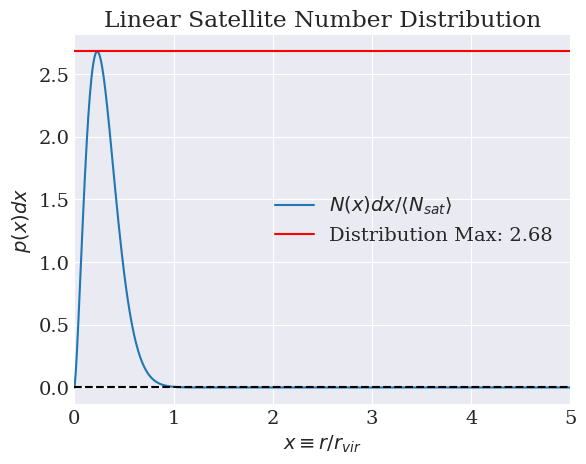
\includegraphics[width=0.8\textwidth]{results/pxdx.png}
    \caption{Analytical distribution of the number of satellite galaxies in a shell around a massive galaxy with thickness $dr$ at radius $r$, described by equation \ref{eq:pxdx}.}
    \label{fig:pxdx_distribution}
\end{figure}

In this work we will use rejection sampling to simulate this distribution. The implementation in this work first generates two random numbers generated using \texttt{32-bit multiply with carry}, we call the first number $x$ and shift it to a uniform distribution in log-space in the range $\left[-4, ^{10}\log(5)\right]$ (corresponding to the range $\left[10^{-4}, 5\right]$ in linear space), and the second we call $y$ and shift it to the range $\left[0, 2.68\right]$ where $2.68$ is the maximum of the distribution given in equation \ref{eq:pxdx} as shown in figure \ref{fig:pxdx_distribution}. If the $\left(x_i, y_i\right)$ point falls below the curve described by equation \ref{eq:pxdx} we accept it, otherwise we reject it\footnote{In the code, we have replaced each $x$ in equation \ref{eq:pxdx} with $10^x$ to account for the fact we sample in log-space.}. After each step we use the last generated random number as \texttt{x0} for the next number. We repeat this entire process, until we have $N = 10^4$ samples in total. We note that rejection sampling is far from the most efficient method to sample a distribution such as this because the majority of possible points in our $\left(x, y\right)$ range will be rejected as is evident in figure \ref{fig:pxdx_distribution}. To slightly combat this we have sampled $x$ in log- instead of linear space which means small values ($<1$) are sampled at a higher rate, and the algorithm finds itself in the "interesting" region of the distribution more often. Nevertheless, on average the rejection sampling algorithm still takes $\sim~6$ attempts (12 random numbers generated) untill it finds an accepted point.

We plot the results from our sampling algorithm as a histogram with 20 equally spaced bins in log-space in figure \ref{fig:gal_pdf}. We divided the height of each bin by $10^3$ to account for the difference between $\left<N_{sat}\right>$ and $N$. We can see in the figure that the analytical distribution, and our sampled distribution match almost perfectly everywhere except the edges. These edges are missing from this plot because the sampler is often unable to sample points in these regions due to the large value for $p(x)dx$ there.

\begin{figure}
    \centering
    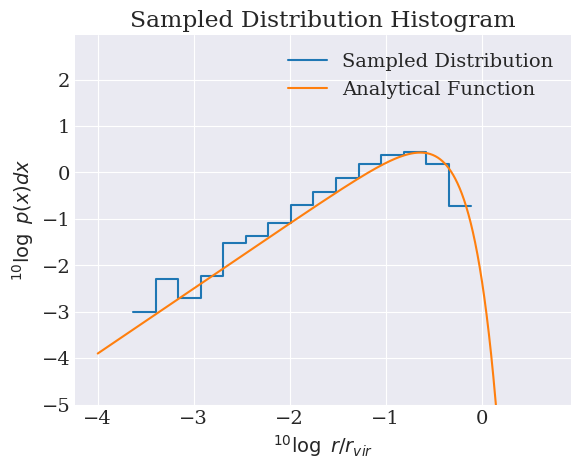
\includegraphics[width=0.8\textwidth]{results/satellite_galaxies_pdf.png}
    \caption{Analytical distribution of satellite galaxies around a massive central overplotted on the same distribution sampled by our rejection algorithm with $N=10^4$ described in the text. The histgoram bin heights are scaled down by a factor $10^3$ to enforce the same normalization.}
    \label{fig:gal_pdf}
\end{figure}

\lstinputlisting[caption={Code to sample the distribution given in this assignment}, linerange={44-89}]{satellite_galaxies.py}

\subsection{Random Selection}

We want to look at the cumulative distribution function (CDF) of the sampled probability distribution shown in figure \ref{fig:gal_pdf}. To do this we first select 100 random satellite galaxies following the criteria given on the handout: each galaxy is selected with equal probabilty, no galaxy is selected twice, and we do not reject any draws. The simple (but maybe relatively overboard) method we use to ensure these criteria are upheld is to first shuffle the array of $10^4$ galaxies in a random order, and then select the first 100.

We perform the random shuffling by generating $10^4$ random numers using our random number generator mentioned earlier, and use these numbers as keys in our \texttt{merge\_sort} algorithm on which to "sort" an array of indices. We then apply these "sorted" indices on the sampled array to shuffle it, and select the first 100 instances. Finally, we sort these 100 galaxies using the same algorithm on their radii directly. We then use this sorted array to plot a CDF, normalized to $1$, and present this in figure \ref{fig:gal_cdf}.

\begin{figure}
    \centering
    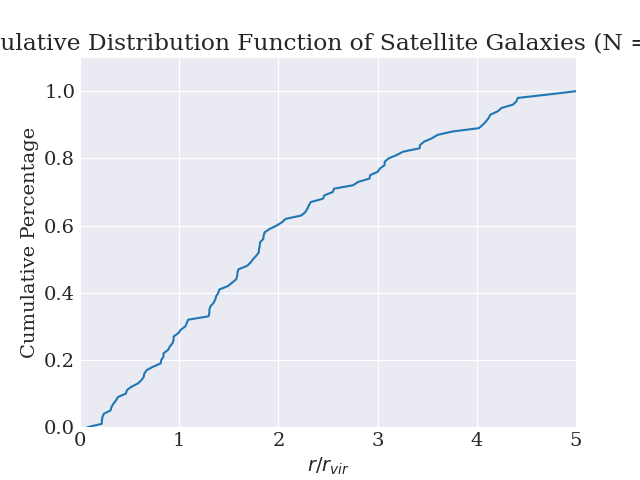
\includegraphics[width=0.8\textwidth]{results/satellite_galaxies_cdf.png}
    \caption{Cumulative distribution function normalized to 1 of $p(x)dx$ sampled using rejection sampling with $N=10^4$, created using only a random subset of 100 satellites.}
    \label{fig:gal_cdf}
\end{figure}

In correspondence with the PDF we saw in figure \ref{fig:gal_pdf}, we can see there are almost no satellites present at either edges of the interval. The most satellite galaxies are found at $\sim x = 0.1$, a result we also saw earlier.

\lstinputlisting[caption={Code used to compute the histogram bins}, firstline={14}]{plotting.py}
\lstinputlisting[caption={Code to generate the CDF presented in this work}, linerange={91-115}]{satellite_galaxies.py}

\subsection{Derivative}

To conclude this section we will look at the derivative of $n(x)$ (equation \ref{eq:nx}, not $N(x)$!) at $x=1$. To compute this derivative we have used Ridder's Method with $h_{start} = 0.1$. Similarly to the Romberg integration earlier, we cannot choose $h_{start} = 1$ because then we would have to sample $n(x=0)$, where the function is not defined. In agreement with the assignment, we set our target accuracy at $10^{-12}$. This means we stop if our uncertainty, defined as the absolute difference between the current and previous best estimates, drops below this threshold. We compare our findings to the analytical derivative of $n(x)$ which we find to be

\begin{equation}
    \frac{dn}{dx}_{(analytical)} = -A\left<N_{sat}\right>\exp\left[-\left(\frac{x}{b}\right)^c\right]~\frac{b^3\left(\frac{x}{b}\right)^a\left(c\left(\frac{x}{b}\right)^c - a + 3 \right) }{x^4}
\end{equation}

Now comparing the two results, using Ridder's Method we find

\begin{equation*}
    \frac{dn}{dx}_{(ridder)} = -0.625328061833 \pm 2.220 \times 10^{-14}
\end{equation*}

While analytically we find

\begin{equation*}
    \frac{dn}{dx}_{(analytical)} = -0.625328061833
\end{equation*}

These two values match exactly up to 12 digits, indicating the strength of the numerical differentiator implemented here.

\lstinputlisting[caption={Analytical derivative function, and code to use Ridder's Method}, linerange={117-126}]{satellite_galaxies.py}
